% !TEX root = ../dissertacao.tex
\chapter{Síntese Física como estudo de caso}
\label{cap:caracterizacaoSinteseFisica}

% este capitulo visa caracterizar e identificar quais algoritmos de physical design podem se beneficiar do uso do modelo de programação orientado a dados

%     \section{escolha dos algoritmos}      
%         apresentar o conjunto de características que foi identificado na seção anterior
%         discutir quais dessas características são benéficas no modelo DOD e quais destas não se aplica ao modelo DOD (ILP)
%         apresentar quais problemas este trabalho irá avaliar

%     \section{DOD em algoritmos de Physical Design}
%     como aplicar o dod em problemas
%         Problema A - limites do chip
%             como seria modelado OOD
%             como seria modelado DOD
%         Problema B - interconexão
%             como seria modelado OOD
%             como seria modelado DOD
%         Problema C - cluster
%             como seria modelado OOD
%             como seria modelado DOD
%         Problema D - roteamento das nets
%             como seria modelado OOD
%             como seria modelado DOD

Este capítulo caracteriza os algoritmos empregados na etapa de síntese física do fluxo de projeto de \acp{ic} segundo a metodologia \textit{standard cells}, enfatizando a organização dos dados de cada algoritmo.
% Com estas características, será possível eleger um subconjunto de algoritmos que representam a síntese física.
A Figura~\ref{fig:exemplo_fluxo_com_algoritmos} apresenta o fluxo de projetos de um \ac{ic} com um maior detalhamento para a etapa de síntese física. 
A síntese física é responsável por instanciar todos os elementos (células) do circuito com suas respectivas informações geométricas, posicionar estes em uma região 2-D e realizar as interconexões necessárias. O resultado da síntese física é um conjunto de especificações que serão posteriormente verificadas, antes de serem utilizadas na fabricação do \acp{ic}~\cite{kahng2011vlsi}.
% Para cada etapa pertencente da síntese física são explanados os principais algoritmos e técnicas de programação utilizados.
% Note que alguns algoritmos, como por exemplo Simulated Annealing (SA)~\cite{russell2009artificial}, são utilizados em diversas fases deste fluxo.

\begin{figure}[!b]
    \centering
    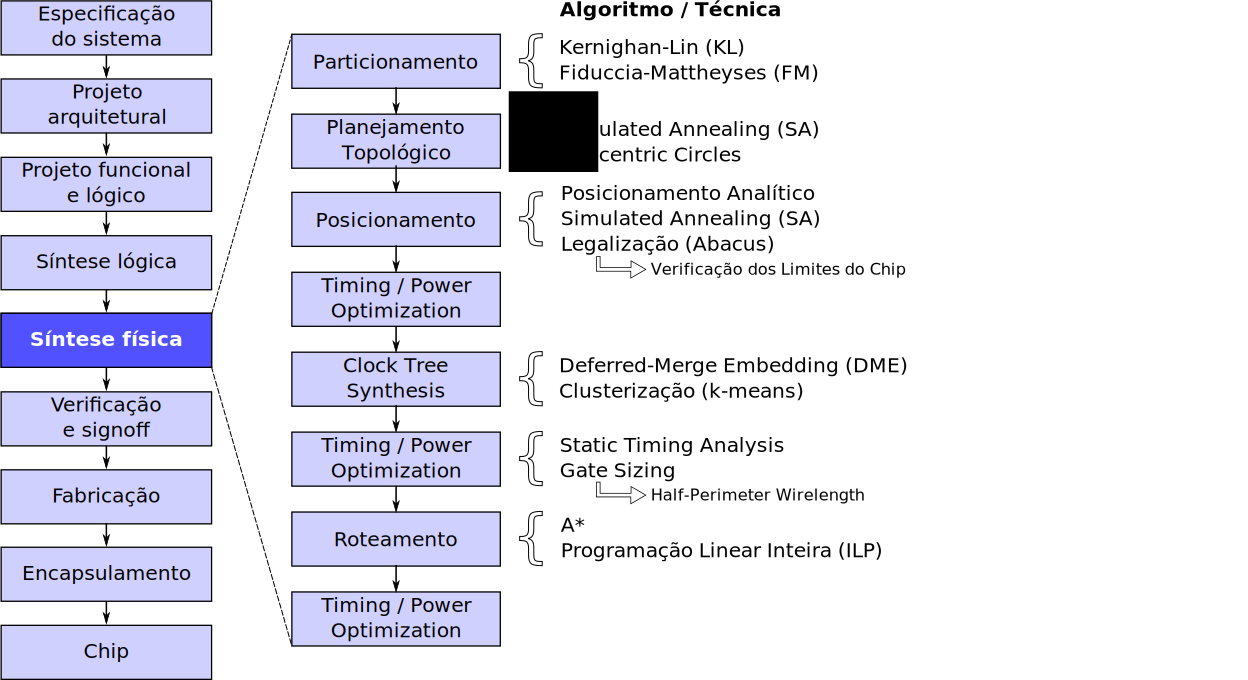
\includegraphics[width=\textwidth]{img/caracterizacao/exemplo_fluxo_com_algoritmos.pdf}
    \caption[Etapas da síntese física]{Etapas da síntese física com seus respectivos algoritmos/técnicas. Figura adaptada de~\citeonline{kahng2011vlsi}.}
    \label{fig:exemplo_fluxo_com_algoritmos}
\end{figure}

O \textbf{particionamento} é a primeira etapa da síntese física e tem como objetivo dividir o \ac{ic} em sub-circuitos para minimizar o número de interconexões entre estas partições \cite{kahng2011vlsi}. Para resolver este problema de particionamento, existem dois algoritmos clássicos: \ac{kl}~\cite{kernighan1970efficient} e \ac{fm}~\cite{fiduccia1988linear}.

% O algoritmo KL opera sobre uma representação do circuito modelada através de um grafo $G(V, E)$. Os nodos $e \in E$ deste grafo representam as células do circuito, enquanto, as arestas $v \in V$ modelam as conexões entre as células. Dado este grafo $G$, cujo $|V| = 2n$ e cada aresta $v$ possui o mesmo peso, o algoritmo KL particiona o conjunto de nodos $V$ em dois conjuntos disjuntos ($A$ e $B$) de mesmo tamanho, isto é, $|A| = |B| = n$.
% Para realizar este particionamento, o algoritmo KL realiza a troca de dois nodos $e_1 \in A$ e $e_2 \in B$ entre as partições com objetivo de minimizar o número de arestas intersectadas pelas partições. Após esta troca, os nodos ($e_1$ e $e_2$) são fixados para prevenir movimentos reversos.

% O algoritmo FM também opera sobre uma modelagem do circuito representada em grafo. Este algoritmo oferece melhorias significativas perante o algoritmo KL. Nele, as células podem ser movidas independentes entre as partições, o que facilita o particionamento de conjuntos de tamanhos distintos. O algoritmo FM utiliza a área da célula no cálculo do peso das arestas do grafo. Esta consideração leva a mover primeiro as células com menor área e visa reduzir a perturbação gerada pelo particionamento. A complexidade do algoritmo FM é $\mathcal{O}(|Pins|)$.

Os dois algoritmos, \ac{kl} e \ac{fm}, representam o circuito através de um grafo $G(V, E)$ , onde os nodos $v \in V$ representam as células e as arestas $e \in E$ modelam as conexões entre as células. Dado este grafo $G$, cujo $|V| = 2n$ e cada aresta $e$ possui o mesmo peso, o algoritmo \ac{kl} particiona o conjunto de nodos $V$ em dois conjuntos disjuntos ($A$ e $B$) de mesmo tamanho, isto é, $|A| = |B| = n$.
Para realizar este particionamento, o algoritmo \ac{kl} realiza a troca de dois nodos $v_1 \in A$ e $v_2 \in B$ entre as partições, com objetivo de minimizar o número de arestas intersectadas pelas partições. Após esta troca, os nodos ($v_1$ e $v_2$) são fixados para prevenir movimentos reversos.
O algoritmo \ac{fm} oferece melhorias significativas perante o algoritmo \ac{kl}. Nele, uma única  célula pode ser movida entre as partições, o que facilita o particionamento de conjuntos de tamanhos distintos ($|A| \neq |B|$).
O algoritmo \ac{fm} utiliza a área da célula no cálculo do peso das arestas do grafo. Esta consideração leva a mover primeiro as células com menor área e visa reduzir a perturbação gerada pelo particionamento. 
A complexidade do algoritmo \ac{fm} é $\mathcal{O}(n)$, onde $n = |V|$, ao passo que a complexidade do algoritmo \ac{kl} é $\mathcal{O}(n^2~log~n)$, onde $n = |V|$.


Na etapa de \textbf{planejamento topológico} são definidas as localizações e formas dos módulos pertencentes ao circuito.
Com estas informações, é possível realizar estimativas precoces do comprimento das interconexões (\textit{wirelength}) e atraso. 
Esta análise inicial permite identificar quais blocos precisam de maior otimização nas etapas posteriores do fluxo de projeto do \ac{ic}. 
A etapa de planejamento topológico é tipicamente dividida em três subetapas, quais sejam: \textit{floorplanning}, \textit{pin assignment} e \textit{power planning}.
A subetapa de \textit{floorplanning} determina as localizações e dimensões, com base nas áreas e relações dos módulos, de modo a otimizar o tamanho do chip, reduzir as interconexões e otimizar a temporização do circuito. Para isso, esta etapa avalia diferentes posicionamentos dos módulos pertencentes ao circuito.
O resultado final desta etapa pode ser observado na Figura~\ref{subfig:resultadofloorplan}, onde a área total do \textit{chip} foi minimizada e possui $35$ unidades.
Um possível algoritmo para esta etapa é o \ac{sa}~\cite{russell2009artificial}.

O algoritmo \ac{sa} é iterativo - parte de uma solução inicial ($s_i$) e busca incrementalmente melhorar a função objetivo $F$.
A cada iteração, soluções vizinhas ($S_v$) são consideradas.
Estas soluções vizinhas são obtidas com uma pequena perturbação na solução atual ($S_v = s_a \pm \alpha$).
Para cada $s \in S_v$, se $s$ for melhor que a solução atual ($F(s) < F(s_a)$ assumindo um objetivo de minimização da função objetivo $F$) esta solução é tomada como nova solução atual ($s_a = s$).
Senão, existe uma probabilidade $t$ (chamada de temperatura, por analogia ao processo metalúrgico de recozimento) da solução $s$ ser tomada como solução atual. Esta probabilidade $t$ é reduzida à medida que o algoritmo executa, de forma que o mesmo sempre possui convergência para uma solução ótima local.
% Se esta probabilidade fosse infinitamente reduzida o algoritmo sempre encontraria o ótimo global, porém, isso não é verdade na prática.

\begin{figure}[h!t]
    \centering
    \subfigure[]{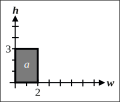
\includegraphics[width=0.3\textwidth]{img/caracterizacao/floorplan/floorplan.pdf} \label{subfig:resultadofloorplan}}
    \subfigure[]{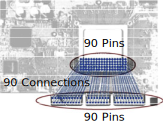
\includegraphics[width=0.3\textwidth]{img/caracterizacao/floorplan/pin_assignment.pdf} \label{subfig:resultadopinAssignment}}
    \subfigure[]{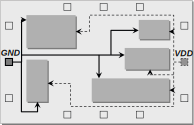
\includegraphics[width=0.32\textwidth]{img/caracterizacao/floorplan/power_planning.pdf} \label{subfig:resultadopowerPlanning}}
    
    \caption[Etapas do planejamento topológico.]{Etapas do planejamento topológico. Retirado de \citeonline{kahng2011vlsi}.}
    \label{fig:etapasPlanejamentoTopologico}
\end{figure}

A subetapa de \textit{pin assignment} conecta as redes de sinais de interface (entradas e saídas) do \ac{ic} com os pinos pertencentes aos blocos internos ao \ac{ic}.
O resultado final desta etapa pode ser observado na Figura~\ref{subfig:resultadopinAssignment}.
A Figura~\ref{fig:concentricCircles} apresenta os principais passos do algoritmo Concentric Circles \cite{koren1972pin, brady1984approach}, um dos principais algoritmos para esta etapa.
Este algoritmo assume que todos os pinos externos (pinos fora do bloco atual) possuem localizações fixas (representados pelos círculos em verde na Figura~\ref{subfig:concentricCircles::a}). 
O algoritmo utiliza dois círculos concêntricos - o círculo interno mapeia os pinos do bloco atual (fontes dos sinais), ao passo que o círculo externo mapeia os pinos dos demais blocos conectados a este (destinos dos sinais).
Para cada pino, é traçada uma linha do centro do círculo até sua posição, e sua posição é projetada para o respectivo círculo.
Este mapeamento pode ser observado pelos pontos em vermelho na Figura~\ref{subfig:concentricCircles::c}.
O mapeamento inicial é determinado interconectando-se um dado pino fonte e um destino (linha trastejada da Figura~\ref{subfig:concentricCircles::d2}) e mapeando os demais pinos no sentido horário.
O mapeamento de todos os pinos pode ser observado na Figura~\ref{subfig:concentricCircles::g}.
Este processo é repetido para cada combinação de fonte/destino, sendo o melhor mapeamento determinado pela menor distância Euclidiana entre todos os fontes/destinos.
Neste exemplo, o melhor mapeamento para os pinos é o mostrado pela Figura~\ref{subfig:concentricCircles::e}.
Após determinar o mapeamento, este algoritmo conecta os pinos do bloco atual (fontes dos sinais) com os pinos dos demais blocos conectados a este (destinos dos sinais), Este passo é ilustrado pela Figura~\ref{subfig:concentricCircles::f}.

\begin{figure}[h!t]
    \centering
    \subfigure[]{\includegraphics[width=0.3\textwidth]{img/caracterizacao/concentricCircles/a.pdf} \label{subfig:concentricCircles::a}}
    % \subfigure[]{\includegraphics[width=0.32\textwidth]{img/caracterizacao/concentricCircles/b.pdf} \label{subfig:concentricCircles::b}}
    \subfigure[]{\includegraphics[width=0.3\textwidth]{img/caracterizacao/concentricCircles/c.pdf} \label{subfig:concentricCircles::c}}
    \subfigure[]{\includegraphics[width=0.3\textwidth]{img/caracterizacao/concentricCircles/d2.pdf} \label{subfig:concentricCircles::d2}}
    
    \subfigure[]{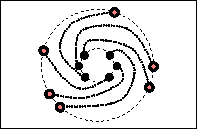
\includegraphics[width=0.3\textwidth]{img/caracterizacao/concentricCircles/g.pdf} \label{subfig:concentricCircles::g}}
    \subfigure[]{\includegraphics[width=0.3\textwidth]{img/caracterizacao/concentricCircles/e.pdf} \label{subfig:concentricCircles::e}}
    \subfigure[]{\includegraphics[width=0.3\textwidth]{img/caracterizacao/concentricCircles/f.pdf} \label{subfig:concentricCircles::f}}
    \caption[Ilustração algoritmo \textit{Concentric Circles}]{Exemplo da execução do algoritmo \textit{Concentric Circles}. Adaptado de \citeonline{kahng2011vlsi}.}
    \label{fig:concentricCircles}
\end{figure}

Na subetapa de \textit{power planning} constrói-se a rede de distribuição de energia, isto é, as redes de \textit{VDD} e de \textit{ground}, de modo a assegurar que cada bloco seja alimentado com a tensão apropriada. A Figura~\ref{subfig:resultadopowerPlanning} apresenta o resultado desta etapa.

A etapa de \textbf{posicionamento} (\textit{placement}) é responsável por encontrar as posições e orientações de todos os elementos do circuito numa superfície planar.
Este posicionamento deve respeitar uma série de restrições (as células não podem se sobrepor, todas as células devem estar alinhadas com as linhas e colunas do circuito, as células devem respeitar a linha de alimentação, sendo rotacionadas quando necessário) e minimizar uma gama de objetivos (comprimento das interconexões, densidade do circuito).
A etapa de posicionamento é dividida em três subetapas: posicionamento global, legalização e posicionamento detalhado.
O posicionamento global negligencia algumas restrições (sobreposição e alinhamento das células) para simplificar o problema e viabilizar o posicionamento de \acp{ic} com milhões de células.
O principal objetivo nesta etapa é a redução das interconexões,  enquanto procura equalizar a densidade de portas pelo circuito.
Para encontrar o local ideal de cada célula no circuito, são utilizadas técnicas analíticas para minimizar a função objetivo~\cite{tsay1988proud, eisenmann1998generic, Lin2013Polar}.
Uma técnica amplamente utilizada nesta subetapa é o algoritmo \ac{sa}. 

Como as técnicas de posicionamento global negligenciam algumas métricas, a etapa subsequente, denominada \textbf{legalização}, tem como propósito resolver as violações introduzidas pelo posicionamento global, tais como: sobreposições de células, e alinhamento das células com a grade de alimentação, linhas e colunas do circuito.
Existem diversos algoritmos para a legalização de \acp{ic}, sendo o Abacus~\cite{spindler2008abacus} um dos mais utilizados.
Abacus é um algoritmo de programação dinâmica que legaliza as células do circuito uma de cada vez, posicionando-as nas linhas que minimizam seu deslocamento com relação às posições encontradas pelo posicionamento global.

A etapa de legalização pode perturbar a solução encontrada pelo posicionamento global. Então, após a legalização é aplicada uma etapa de posicionamento detalhado.
Esta etapa reposiciona algumas células do circuito, otimizando métricas específicas, como por exemplo, atraso do circuito e densidade das células.
Para esta etapa são utilizados algoritmos iterativos que refinam incrementalmente o posicionamento das células críticas do circuito.

Com todas as células do circuitos posicionadas e legalizadas a etapa de \textbf{clock tree synthesis} (geração da árvore de relógio) irá agrupar elementos  sequenciais sincronizados pelo menos sinal de relógio e planejar a rede de relógio do \ac{ic}.
Um dos algoritmos clássicos para o agrupamento de elementos conectados pela mesma rede de relógio é denominado K-\textit{means}~\cite{selim1984k}.
O algoritmo inicia criando $k$ \textit{clusters} (grupos) com centros aleatórios. Em seguida, na etapa de assinalamento, todos os elementos sequenciais são assinalados para o \textit{cluster} mais próximo.
Após assinalar todos os elementos, o centro do \textit{cluster} é ajustado para que corresponda ao centro de massa dos elementos que o pertencem. Estas duas etapas são repetidas por um número fixo de vezes ou até que os centros dos \textit{clusters} convirjam.

Para gerar a rede de relógio, dentre os algoritmos clássicos temos como exemplo o \ac{dme}~\cite{boese1992zero}.
Este algoritmo é baseado no conceito de divisão e conquista e em tempo linear constrói, a topologia de conexão no plano de Manhattan para criar uma árvore de relógio com \textit{clock skew} zero, minimizando o comprimento de fio das interconexões de relógio.
\textit{Clock Skew} é a máxima diferença, no tempo de chegada (\textit{arrival time}) do sinal de relógio, entre todos os elementos sequenciais. Se $t(u,v)$ representa o atraso na chegada do sinal de relógio entre os elementos sequenciais $u$ e $v$, o \textit{skew} de uma rede de relógio $T$ é calculado segundo a Equação \ref{eq.skew}.
\begin{equation} \label{eq.skew}
	 \displaystyle \operatorname{\textit{skew}(T)} = \max_{S_{i}, S_{j} \in S} | t(S_{0},S_{i})-t(S_{0},S_{j})|
%	 \displaystyle \operatorname{\textit{skew}(T)} = \max_{i,j \in S} | at_i^L - at_j^L|
\end{equation} 

A etapa de \textbf{roteamento} é responsável por criar todas as interconexões de sinais (\textit{nets}) do \ac{ic}.
% Durante a etapa de \textbf{roteamento} todas as interconexões de sinais (\textit{nets}) devem ser estabelecidas. 
Esta etapa é subdividida em dois passos: 1) roteamento global; 2) roteamento detalhado.
No roteamento global a área do circuito é dividida segundo uma grade, sendo cada divisão da grade referenciada por gcell.
A capacidade de cada gcell corresponde ao número de interconexões que podem ser roteadas na porção do circuito por ela representada.
O modelo utilizado para representar estas informações de forma computacional é um Grafo G(V, E) no qual cada vértice $v \in V$ representa uma gcell e cada aresta $(u, v) \in E$ representa a capacidade da gcell $u$ rotear um sinal para a gcell vizinha $v$.
Então, um algoritmo de busca em grafo, como por exemplo o algoritmo A*~\cite{russell2009artificial}, é usado para identificar as gcells pelas quais a interconexão irá passar, a fim de modelar uma conexão entre um par de pinos.
% Um algoritmo capaz de definir por quais gcells a interconexão passa é o $A*$~\cite{russell2009artificial}.
Na etapa de roteamento detalhado são definidas as trilhas de roteamento, vias e camadas de metal para cada segmento de interconexão do circuito.
Estas definições devem respeitar todas as regras de desenho do leiaute estabelecidas para uma dada tecnologia de fabricação~\cite{kahng2011vlsi}.
Para isso, é definido um conjunto de equações a serem solucionadas por meio de \ac{ilp}.
Entre os roteadores clássicos baseados em \ac{ilp} estão Sidewinder~\cite{hu2008sidewinder} e BoxRouter~\cite{cho2007boxrouter}.


Ao longo do fluxo de projeto do \ac{ic}, a etapa de \textbf{\textit{timing/power optimization}} é responsável por garantir o atendimento da especificação de consumo de energia e da frequência de operação alvo, o que requer estimativas precisas de atraso. 
Para estimar o atraso do circuito, a \textit{Static Timing Analysis}~(STA)~\cite{srivastava2006statistical, chadha2009static} propaga os atrasos das células e interconexões para identificar os locais com violações temporais.
Para isto, o circuito é modelado como um grafo G(V, E) no qual cada vértice $v \in V$ representa uma célula do circuito e cada aresta $(u, v) \in E$ representa a interconexão entre a célula $u$ e a célula $v$. 
Uma vez identificadas as violações temporais, diferentes heurísticas são aplicadas para resolvê-las.
% Esta etapa é denominada \textit{Timing/Power Optimization} e possui dois grandes passos: \textit{Static Timing Analysis}~(STA)~\cite{srivastava2006statistical, chadha2009static} e \textit{Gate Sizing}.
% A análise consiste em propagar os atrasos das células e interconexões para identificar os locais com violações temporais.
% A etapa de \textit{Gate Sizing} é responsável por corrigir as violações temporais identificadas anteriormente.
% Estas correções são realizadas com a alteração do tamanho das células (uma biblioteca standard-cell tipicamente fornece a  mesma célula com diferentes tamanhos que correspondem a diferentes \textit{drive strengths}~\footnote{\textit{Drive strengths} é a quantidade de corrente que uma célula pode fornecer em seu chaveamento.}), a inserção de \textit{buffers} e a reestruturação da \textit{netlist}.

% sumarização da síntese física

A Tabela~\ref{tab:caracteristicasSinteseFisica} enumera as etapas da síntese física e caracteriza os algoritmos e as técnicas empregadas em cada etapa. Ela também relaciona as estruturas de dados usadas pelos referidos algoritmos e técnicas.
% Para cada etapa são descritos seus algoritmos e/ou técnicas bem como suas estruturas de dados e/ou métodos utilizados. 
Note que diversos algoritmos/técnicas utilizam estruturas de dados elementares, como por exemplo: arranjos, pilhas, filas, conjuntos, entre outras.
Algumas outras etapas representam as informações do circuito por meio de grafo.
Também existem etapas que fazem uso de outros métodos de programação, tais como: Programação Linear, Programação Quadrática e Programação Dinâmica.

% Please add the following required packages to your document preamble:
% \usepackage{booktabs}
% \usepackage{multirow}
% \usepackage{graphicx}
\begin{table}[h!b]
\centering
\caption{Caracterização da Síntese Física}
\label{tab:caracteristicasSinteseFisica}
\resizebox{\textwidth}{!}{%
\begin{tabular}{@{}lll@{}}
\toprule
Etapa                                                                                  & Algoritmo / Técnica            & Estrutura de Dados / Método      \\ \midrule
\multirow{2}{*}{Particionamento}                                                       & Kernighan-Lin (KL)             & Grafo                            \\
                                                                                       & Fiduccia-Mattheyses (FM)       & Grafo                            \\ \midrule
\multirow{2}{*}{Planejamento Topológico}                                               & Simulated Annealing (SA)       & Elementar                        \\
                                                                                       & Concentric Circles             & Elementar                        \\ \midrule
\multirow{3}{*}{Posicionamento}                                                        & Posicionamento Analítico       & Programação Linear               \\
                                                                                       & Simulated Annealing (SA)       & Elementar                        \\
                                                                                       & Abacus                         & Programação Dinâmica             \\ \midrule
\multirow{2}{*}{\begin{tabular}[c]{@{}l@{}}Timing / Power\\ Optimization\end{tabular}} & Static Timing Analysis (STA)   & Grafo                            \\
                                                                                       & Gate Sizing                    & Grafo                            \\ \midrule
\multirow{2}{*}{Clock Tree Synthesis}                                                  & Deferred-Merge Embedding (DME) & Elementar                        \\
                                                                                       & K-means                        & Elementar                        \\ \midrule
\multirow{2}{*}{Roteamento}                                                            & A*                             & Grafo                            \\
                                                                                       & Sidewinder                     & Programação Linear Inteira (ILP) \\ \bottomrule
\end{tabular}%
}
\end{table}

% Please add the following required packages to your document preamble:
% \usepackage{multirow}
% \usepackage{graphicx}
% \begin{table}[]
% \centering
% \caption{Caracterização da Síntese Física}
% \label{tab:caracteristicasSinteseFisica}
% \resizebox{\textwidth}{!}{%
% \begin{tabular}{lll}
% \hline
% Etapa                                                                                  & Estratégia                     & Organização dos Dados            \\ \hline
% \multirow{2}{*}{Particionamento}                                                       & Kernighan-Lin (KL)             & Grafo                            \\
%                                                                                       & Fiduccia-Mattheyses (FM)       & Grafo                            \\ \hline
% \multirow{2}{*}{Planejamento Topológico}                                               & Simulated Annealing (SA)       &                                  \\
%                                                                                       & Concentric Circles             &                                  \\ \hline
% \multirow{3}{*}{Posicionamento}                                                        & Posicionamento Analítico       & Programação Linear               \\
%                                                                                       & Simulated Annealing (SA)       &                                  \\
%                                                                                       & Abacus                         & Programação Dinâmica             \\ \hline
% \multirow{2}{*}{\begin{tabular}[c]{@{}l@{}}Timing~/~Power Optimization\end{tabular}} & Static Timing Analysis (STA)   & Grafo                            \\
%                                                                                       & Gate Sizing                    & Grafo                            \\ \hline
% \multirow{2}{*}{Clock Tree Synthesis}                                                  & Deferred-Merge Embedding (DME) &                                  \\
%                                                                                       & K-means                        &                                  \\ \hline
% \multirow{2}{*}{Roteamento}                                                            & A*                             & Grafo                            \\
%                                                                                       & Sidewinder                     & Programação Linear Inteira (ILP) \\ \hline
% \end{tabular}%
% }
% \end{table}


% Please add the following required packages to your document preamble:
% \usepackage{booktabs}
% \usepackage{multirow}
% \usepackage{graphicx}
% \begin{table}[]
% \centering
% \caption{My caption}
% \label{my-label}
% \resizebox{\textwidth}{!}{%
% \begin{tabular}{@{}lll@{}}
% \toprule
% Etapa                                    & Estratégia                     & Organização dos Dados            \\ \midrule
% \multirow{2}{*}{Particionamento}         & Kernighan-Lin (KL)             & Grafo                            \\
%                                          & Fiduccia-Mattheyses (FM)       & Grafo                            \\ \midrule
% \multirow{2}{*}{Planejamento Topológico} & Simulated Annealing (SA)       &                                  \\
%                                          & Concentric Circles             &                                  \\ \midrule
% \multirow{3}{*}{Posicionamento}          & Posicionamento Analítico       & Programação Linear               \\
%                                          & Simulated Annealing (SA)       &                                  \\
%                                          & Abacus                         & Programação Dinâmica             \\ \midrule
% \multirow{2}{*}{Clock Tree Synthesis}    & Deferred-Merge Embedding (DME) &                                  \\
%                                          & K-means                        &                                  \\ \midrule
% \multirow{2}{*}{Roteamento}              & A*                             & Grafo                            \\
%                                          & Sidewinder                     & Programação Linear Inteira (ILP) \\ \midrule
% \multirow{2}{*}{Timing Closure}          & Static Timing Analysis (STA)   & Grafo                            \\
%                                          & Gate Sizing                    & Grafo                            \\ \toprule
% \end{tabular}%
% }
% \end{table}

Com isso é possível eleger um subconjunto, dentre os algoritmos/técnicas empregados no fluxo da síntese física, que cubra as características mais relevantes de todos os problemas encontrados em tal fluxo.
Desta forma, para este trabalho os seguintes algoritmos/técnicas foram escolhidos como estudos de caso:
\begin{enumerate}
    \itemsep0em
    \item \textbf{Verificação dos limites do chip}: pertencente à etapa de legalização do posicionamento de um \ac{ic}. Este estudo de caso representa tarefas simples e com estruturas de dados elementares. Porém, estas são executadas muitas e muitas vezes durante o fluxo de projeto.
    \item \textbf{Estimativa do comprimento de interconexões}: pertencente às etapas de posicionamento e \textit{timing/power optimization}. Esta tarefa depende de diversas informações, 
    tradicionalmente separadas em diversos módulos. Possui baixa intensidade aritmética e utiliza estrutura de dados elementares.
    \item \textbf{Clusterização de registradores}: Pertencente à etapa de \textit{Clock Tree Synthesis}. Esta tarefa necessita de poucas informações e utiliza estruturas de dados elementares. Porém, realiza um alto número de operações aritméticas. 
    \item \textbf{Roteamento global}: pertencente à etapa de roteamento do \ac{ic}. Esta etapa opera sobre um grafo que representa o leiaute do circuito e visa determinar o percurso de cada interconexão do circuito.
\end{enumerate}

Não foram analisadas tarefas que utilizam Programação Linear e Programação Quadrática pois grande parte do esforço nestes modelos concentra-se na solução de um sistema de equações matemáticas.
Estas equações são resolvidas por meio de solucionadores matemáticos externos, os quais possuem como entrada estruturas de dados previamente definidas.
Isto torna impossível aplicar outra organização (por exemplo \ac{dod}) nos dados internos destes resolvedores.
Com isso, alterar a organização dos dados numa pequena parcela da tarefa provavelmente não surtiria efeito sobre o contexto global da tarefa.

Por limitação do escopo deste trabalho, não foram analisadas tarefas que fazem uso de Programação Dinâmica.
Por outro lado, as características encontradas nos algoritmos/técnicas selecionados também estão presentes em algoritmos que resolvem problemas de diversos outros domínios de aplicação, o que permite, em certa medida, especular-se sobre a generalização das conclusões a serem obtidas por meio dos experimentos realizados neste trabalho e apresentados no Capítulo~\ref{cap:resultados}.
